\begin{section}{Informe T\'ecnico}

\begin{subsection}{Introducci\'on}

El objetivo de este trabajo práctico es estudiar las bases de datos NoSQL de tipo Key/Value Store. Nos centraremos en sus características distintivas y ahondaremos en sus ventajas y desventajas en comparación a otras soluciones NoSQL. Luego presentaremos varias implementaciones de la tecnología y qué usos se les da a cada una.

\end{subsection}

\begin{subsection}{Conceptos Básicos}

Las bases de datos Key/Value Store permiten recuperar y guardar datos mediante una clave. La base de datos es indiferente sobre los datos almacenados, es decir no tiene conocimiento sobre su estructura o contenido (no existe un schema), ya que para la base de datos, los valores almacenados no son más que una tira de bytes. En una visión simplificada, las bases de datos Key/Value Store no son más que una tabla de hash. \\

Sus beneficios principales son que escala muy fácil y que, de usarse correctamente, es posible aumentar mucho la performance de un sistema. Además, las tecnologías que implementan Key/Value Store permiten que sea fácil que la base de datos sea distribuida, que se auto-replique, que sean descentralizadas, que los datos se particionen automáticamente y que sean muy performantes(algunas se implementan sobre memoria RAM).\\

Los valores en Key/Value Store se dice que son opacos pues carecen de una estructura definida. A diferencia de otras bases de datos NoSQL basadas en documentos, en las que se puede indexar y consultar valores de atributos, Key/Value Store presenta una limitación importante: no es posible consultar valores de atributos. Como no existen objetos con atributos sino que los objetos son tiras de bytes, los objetos deben ser accedidos mediante una key, la cual es necesario conocer y luego de obtener el objeto el cliente debe saber interpretar los datos contenidos en él.\\

Otra limitación, es que se debe especificar una clave para agregar un nuevo valor, característica que no comparte con las bases de datos documentales, en las que se pueden agregar documentos y la base de datos se encarga de crear la clave.\\

Las bases de datos Key/Value Store son las bases de datos NoSQL más simples, al menos desde el punto de vista de su estructura de datos e interfaz. Todas exponen una variación de la siguiente API:\\ \\
\\
\textbf{void} Put(string key, byte[ ] data);\\
\textbf{byte[ ]} Get(string key);\\
\textbf{void} Remove(string key);\\ 

Los datos en la base de datos son simples blobs, y el cliente es el encargado de interpretar los datos y conocer las keys donde está almacenada la información necesaria.\\

A continuación describimos los conceptos fundamentales de las bases de datos aplicados a Key/Value Store:

\begin{itemize}

\item \textbf{Concurrencia} -  En Key/Value Store, la concurrencia solo se aplica a una clave y suele ser de tipo de ‘escrituras optimistas’ o ‘consistencia eventual’. En los sistema altamente escalables, las escrituras optimistas no suelen ser posibles, pues el costo de chequear que los valores no cambiaron puede ser muy alto si el valor en sí fue replicado en otras máquinas. Por lo tanto lo más común es ver sistemas en los que se usa consistencia eventual.

\item \textbf{Consultas} - No hay forma de realizar una consulta en Key/Value Store, excepto usando la clave. Ni siquiera suele ser posible hacer consultas usando rangos de claves.

\item \textbf{Schema} -  Key/Value Store no permite definir schemas. Pero se podría decir que el esquema consiste en 2 atributos Key y Value, siendo Key un string y Value un blob. 
	
\item \textbf{Escalado} - La forma más simple de escalado es dividir el espacio de claves entre los nodos. De esa manera el valor de una clave estaría almacenada en un único servidor. Eso facilita las cosas, pero tiene la limitante de que si un nodo se cae se pierden los datos. Otra forma es usar replicación.
	
\item \textbf{Replicación} -  La replicación se puede hacer desde el sistema de almacenamiento o por el cliente(escribiendo a múltiples servidores). La replicación introduce el problema de versionado de datos divergente. Esto consiste en que dos nodos pueden creer que el valor asociado a una cierta clave difiere. Resolver eso puede ser complejo y se suele tomar la última versión o dejar que el cliente resuelva los conflictos.
	
\item \textbf{Usos} - Key/Value Store es usado en muchos sistemas de almacenamiento, principalmente para optimizar las consultas. Cosas como los perfiles de usuario, sesiones de usuario, carritos de compra, etc. Notar, que en todos esos casos, se almacena todo el conjunto de datos como un único valor, lo cual facilita manipular esos valores(una única solicitud para escribir o leer) y también no suele ser más fácil, que en otros sistemas, resolver problemas de concurrencia pues el conflicto es sobre una única clave.

\end{itemize}

\end{subsection}

\begin{subsection}{CAP Theorem}

En el mundo de NoSQL es común referirse al CAP Theorem como una de las razones por las cuales las bases de datos usan consistencia eventual. Básicamente el teorema sostiene que dadas tres propiedades: consistencia, disponibilidad y partición (tolerancia a fallos), una base de datos distribuida solo puede garantizar dos de ellas.\\

Consistencia significa que los datos a lo largo de todo un cluster son iguales con lo cual es posible leer y escribir de cualquier nodo. Disponibilidad quiere decir que es posible acceder a un cluster aunque alguno de los nodos del mismo no esté disponible. Partición implica que un cluster continúe funcionando a pesar de que la comunicación entre dos nodos esté caída.\\

Supongamos que tenemos dos nodos X e Y de un cluster C y que la comunicación entre X e Y se cae de manera que no pueden sincronizarse. En este punto tenemos dos posibilidades según el CAP Theorem. O bien permitimos que los nodos estén desincronizados con lo cual sacrificamos la consistencia, o bien damos de baja el cluster con lo que perdemos la disponibilidad. Las posibles combinaciones son: \\

\textbf{CA:} datos consistentes entre todos los nodos (siempre y cuando estén online) y posibilidad de leer y escribir de cualquier nodo y estar seguro de que los datos son los mismos. Sin embargo, si llegase a ocurrir una pérdida de comunicación entre dos nodos estos no serán capaces de re-sincronizarse cuando la comunicación se restablezca.\\

\textbf{CP:} los datos son consistentes entre todos los nodos y se mantiene la tolerancia a la partición (previniendo desincronización de los datos) a cambio de que se pierde la disponibilidad cuando un nodo se cae.\\

\textbf{AP:} los nodos se mantienen online aunque haya falla de comunicación entre ellos y se re-sincronizan cuando la comunicación falla y se restablece. Sin embargo, no podemos garantizar que todos los nodos tengan los mismos datos.\\

\end{subsection}
\end{section}

\pagebreak

\begin{section}{Ejemplos de bases de datos que usan Key-Value}

La idea aquí es presentar diversos ejemplos de bases de datos que utilizan Key/Value Store y compararlas en términos de consistencia, transacciones, querys, estructuras de datos y escalabilidad.

\begin{subsection}{Dynamo}
	
La base de datos Dynamo fue creada por Amazon. Amazon la describe como \textit{“a highly available key-value storage system that some of Amazon’s core services use to provide an ‘always-on’ experience”}. Este servicio no está directamente expuesto al usuario final, como otros tantos servicios de \textit{Amazon}, sino que es usada internamente para dar soporte a otras tecnologías como \textit{Amazon Web Services(S3)}. \\

La API de Dynamo comparte la interfaz común con los sistemas Key/Value Store. El método get se usa para obtener un valor y put para establecer un valor. Pero incorpora el concepto de context a ambos métodos, que consiste en metadata acerca del valor opaco. De manera que al ejecutar get(key) se obtiene el valor asociado a la clave o todas las réplicas asociadas a la clave junto al context(en caso de que haya versiones conflictivas). La interfaz de put difiere, y es de la siguiente manera: put(key, context, value). O sea que el context se almacena junto con el valor. \\

	El contexto es usado por el sistema para asistir en la resolución de conflictos que surgen al particionar los datos, distribuirlos y tener distintas versiones de los datos al mismo tiempo. Por ejemplo una de las cosas que se guardan en el context es la versión de los datos que luego se usa para decidir con que datos quedarse o en caso de ser necesario hacer un merge de los datos.

\begin{subsubsection}{Algoritmo de partición}
Uno de los métodos que Dynamo usa para permitir el escalado es su algoritmo de particionamiento. Este algoritmo usa consistent hashing para distribuir la carga a través de múltiples servidores. \\

	Consistent hashing funciona de la siguiente manera: cada nodo es asignado un valor aleatorio en un rango de valores que wrappean como formando un ‘anillo’. Luego cada objeto es asignado a un nodo haciendo hashing de la key, y obteniendo una posición dentro del anillo y luego, moviéndose hacia delante en sentido horario, da con el primer nodo que tenga posición mayor a la posición del objeto. La principal ventaja de este mecanismo es que si se cae un nodo o se agrega uno nuevo, solo se ven a afectados los vecinos inmediatos y todos los demás objetos se mantienen sin cambios.\\
	
	Consistent hashing presenta un problema: al asignar las posiciones de los nodos de forma aleatoria, la distribución de los datos puede no ser de forma uniforme. Para solucionar ese problema, Dynamo usa Consistent hashing con ‘nodos virtuales’. Esta variación consiste en que cada vez que un nodo es agregado, se crean múltiples nodos virtuales correspondientes al nuevo nodo, cada uno con una posición aleatoria dentro del anillo. De esta manera, al sacar un nodo, los datos no recaen todos sobre el nodo adyacente, sino sobre varios, y de la misma forma cuando se agrega un nuevo nodo, los datos se redistribuyen de manera uniforme.
	\\
\end{subsubsection}

\begin{subsubsection}{Replicación}
	Dynamo también permite replicación. El mecanismo por el cual hace replicación consiste en que por cada key se selecciona un ‘nodo coordinador’ (es el nodo correspondiente al hash de la key en el anillo) y este se encarga de replicar los datos en los N-1 nodos siguientes en sentido horario y quedándose él también con una copia.\\

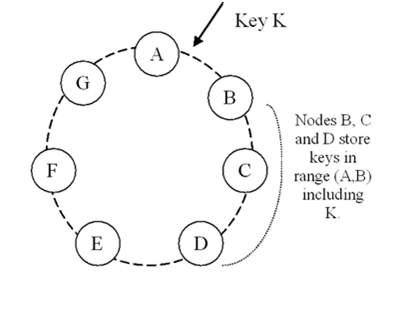
\includegraphics[scale=1]{imgs/dynamo}
	
En caso de usar nodos virtuales, el nodo coordinador se asegura de saltear nodos repetidos, para que el mismo nodo no tenga replicados los datos. \\

\end{subsubsection}

\begin{subsubsection}{Versionado de los datos}

Dynamo provee consistencia eventual, lo cual permite que las actualizaciones se propaguen a todas las réplicas de forma asincrónica. Hay ocasiones en que pueden surgir inconsistencias, si se producen actualizaciones distintas a dos o más réplicas. Dynamo trata esos casos usando versionado de objetos. La versión de un objeto se guarda en el contexto del objeto. Cuando un nodo recibe un objeto con versiones distintas intenta reconciliarlo comparando las versiones y quedándose con la más nueva, si es posible. En caso de no ser posible(porque sucedió branching de las versiones), cuando un cliente pida el objeto, obtendrá todas las versiones del objeto con sus respectivos contextos y será el cliente el encargado de hacer el merge y hacer put() de una nueva versión.\\

	Un caso típico que hace uso del versionado es la funcionalidad del shopping cart. En Dynamo se guarda la información del carrito de compras y cada vez que se agrega o saca un objeto, se hace un put(). Como Amazon no quiere perder ningún ítem que se haya agregado al carrito, entonces siempre se commitean cambios al carrito. Para resolver inconsistencias, se da preferencia a los productos añadidos sobre los eliminados, de modo que al reconciliar distintas versiones de un objeto, pueden reaparecer productos eliminados pero nunca desaparecerán productos añadidos.\\
	
\end{subsubsection}

\begin{subsubsection}{Usos}

	Dynamo es usado por distintos servicios con distintas configuraciones:\\
\begin{itemize}

\item \textbf{Reconciliación de datos usando lógica de negocios:} en esta configuración la reconciliación se hace siguiendo una lógica dada. El mejor ejemplo de este caso es el carrito de compras discutido anteriormente.\\

\item \textbf{Reconciliación basada en timestamp:} la reconciliación se hace en base al timestamp guardado en el contexto: “última escritura gana”. Un buen ejemplo de este caso es la sesión de usuario de un cliente de Amazon.\\

\item \textbf{Motor de lectura de alto rendimiento:} Hay servicios que necesitan hacer muchas lecturas y muy pocas actualizaciones. Los servicios que mantienen los catalogos de productos o los productos promocionales son ejemplos de este caso.\\

\end{itemize}

\end{subsubsection}

\end{subsection}

\begin{subsection}{Riak}

Riak es una base de datos Key/Value, open source, distribuida, con alta disponibilidad, tolerante a fallas y que escala casi linealmente. Soporta un gran volumen de datos y responde fácilmente a medida que crece. Permite almacenar cualquier tipo de datos.\\

Fue construida como una solución a los problemas de Big Data, basándose en el diseño de Dynamo, de Amazon. Actualmente es usada por Github, Comcast, Voxer, Disqus y otras.\\

Riak utiliza buckets y keys para organizar los datos, permitiendo agrupar múltiples key/values en distintos namespaces. \\

La API de Riak comparte la interfaz común de las bases de datos Key/Value: get, put y delete:\\
\\ \\
\textbf{PUT}    /riak/bucket/key \\
\textbf{GET}    /riak/bucket/key \\
\textbf{DELETE} /riak/bucket/key \\

Riak utiliza replicación y particionado. El sistema de replicación está altamente influenciado por el paper de Dynamo y por el CAP Theorem. Al igual que Dynamo, Riak sigue la técnica de consistent hashing que mapea cada key a un rango de particiones que conforman un nodo virtual. Tiene la ventaja de reducir la cantidad de datos que deben ser reequilibrados cuando un nodo se cae. \\

El CAP Theorem asegura que dadas tres propiedades: consistencia, disponibilidad y partición, sólo es posible asegurar dos de estas. Riak decidió realizar un sistema que permitiese jugar con estas limitaciones, siendo posible tunear el nivel de consistencia y disponibilidad de una base de datos según sea necesario. Por ejemplo, es posible definir en cuántos nodos debe ser replicado un objeto y cuántos nodos deben ser escritos o leídos para poder completar exitosamente un pedido. Estos valores son configurables en N/R/W. N es el número de nodos que deben replicarse, R el número de nodos a leer y W el número de nodos que deben ser escritos antes de finalizar una operación. A continuación, un ejemplo:\\

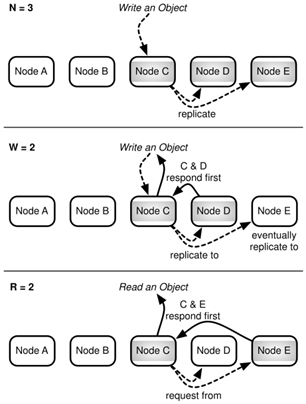
\includegraphics[scale=1]{imgs/riak}

N=3: significa que eventualmente los valores serán replicados en 3 nodos. \\

W=2: significa que es necesario que 2 nodos sean escritos antes de finalizar la operación de escritura, dejando que el nodo restante sea replicado en un futuro. Esto permite operaciones de escritura más rápidos pero, en contraparte, aumentan las probabilidades de que haya lecturas de un valor incoherente en el corto plazo. Seteando W=all (3) podríamos asegurar, prácticamente, que el sistema siempre devuelve valores consistentes, a cambio de operaciones más costosas. \\

R=2: significa que es necesario que 2 nodos sean leídos antes de finalizar la operación de lectura. Esto permite operaciones rápidas a cambio de posibles dirty reads. Para asegurarnos de leer el valor más reciente podríamos leer todos los nodos en donde un valor es replicado siendo estas operaciones muy costosas.\\

En términos generales los valores N/R/W son las formas en que Riak nos permite ofrecer menor consistencia y mayor disponibilidad. \\

Anteriormente mencionamos que los buckets son una forma de segmentar las keys. En verdad, son capaces de más. Riak ofrece la posibilidad de configurar los valores de N$\/$R$\/$W a cada bucket permitiendo que cada uno de estos reaccione distinto frente a operaciones de escritura y lectura. Algunos buckets podrían ser rápidos y poco consistentes o, por el contrario, ser lentos y muy consistentes. El usuario es capaz de configurarlo a gusto según sus necesidades. Otra ventaja de los buckets es la habilidad de hacer que las escrituras cumplan con la conducta que uno espera por medio de hooks que son funciones para ejecutar, ya sea antes o después de que un valor se guarda. De esta manera, sería posible cancelar un commit si, de alguna manera, se considera que los datos son erróneos. \\

Riak utiliza una estructura de datos llamada vector clocks. Esta estructura nos permite decidir, dado un objeto, cuál es el valor más actualizado. Para ello, realiza un seguimiento de los eventos en la base de datos, guardándose cómo y quién modificó un objeto determinado. Hay dos configuraciones posibles: o bien se activa la opción de “last$\_$write$\_$wins” con lo cual se delega la responsabilidad a Riak (decide que la última escritura es válida), o bien se setea “allow$\_$mut” que delega la responsabilidad a la aplicación para que esta decida cómo resolver el conflicto.\\

Resumiendo, Riak está diseñado para otorgar una serie de beneficios en el mundo real. Consistent hashing y vnodes son soluciones para lograr escalado horizontal. N/R/W permite manejar las limitaciones impuestas por el CAP Theorem y, la estructura vector clock, permite un paso más hacia la verdadera consistencia gestionando los conflictos que se producen con una gran carga. \\

\end{subsection}

\begin{subsection}{Redis}

Redis lleva su nombre por REmote DIctionary Server. Aún cuando se la categoriza como key-value store no es puramente tal sino que se la denomina como ‘data structure server’ debido a que soporta diferentes tipos de values. Redis no está limitado únicamente a strings como valores sino que permite estructuras más complejas y tiene operaciones atómicas definidas para estas estructuras. Listas, conjuntos, conjuntos ordenados, hashes, bitmaps y hyperLogLogs son algunos ejemplos de tipos de datos soportados. Puede decirse que Redis es un camino alternativo en la evolución de las key-value stores. \\

Otro feature que presenta Redis común a todos los tipos de values es el llamado Redis expires (Redis expira). Básicamente uno puede setear un timeout para una key, especificando así el tiempo de vida de esa key. Pasado ese tiempo la key se destruye automáticamente, como si el usuario hubiera invocado al comando DEL con dicha key. Este valor de timeout puede setearse con precisión de segundos o milisegundos, es replicada y persiste en disco, e incluso se destruye la key aún si la base se detiene puesto que Redis almacena la fecha exacta en que la clave expira. \\

Redis también soporta transacciones, posibilitando la ejecución de un grupo de comandos de manera atómica. Los scripts de Redis son transaccionales por definición. Pero a diferencia de las bases de datos relacionales, Redis no soporta rollbacks. Si un comando falla durante una transacción, Redis ejecutará el resto de la transacción en lugar de rollbackear. Aun así es preciso destacar que un comando de Redis falla sòlo si tiene un error de sintaxis o se aplica sobre una key que posee el tipo de dato incorrecto. Por ende a fines prácticos, una falla se traduce a un error de programación que muy probablemente se detecte en desarrollo y no en producción. \\

Redis alberga los datos en memoria por lo que está limitado al tamaño de la misma pero sus escrituras y lecturas son a gran velocidad. Así mismo permite persistencia en disco, posiblemente en modo RDB o AOF y no necesariamente habilitado para acceso random sino a modo de append. Suele utilizarse Redis para varios datos pequeños y grandes Blobs en SQL. \\

\end{subsection}

\begin{subsection}{Project Voldemort}

Voldemort es una base de datos no relacional distribuida lo que le permite tener la información disponible y almacenada en distintos lugares sin importar la distancia física que los separe. Esta base de datos aunque no posee una estructura definida para toda la información que contiene de todas formas cumple con las propiedades de ACID.\\

Toda la información que contiene almacenada se replica dependiendo de la cantidad de nodos con que cuenta, mejorando su performance para las lecturas y protegiendo la continuidad de la base independizandola de los posibles fallos de los nodos que la componen. \\

Esta base fue desarrollada y es utilizada actualmente por LinkedIn. Al igual que el resto de las implementaciones noSQL, la API con la que cuenta la aplicación para la alta y modificación de datos es realmente simple:\\
\\
value = store.\textbf{get}(key) \\
store.\textbf{put}(key, value) \\
store.\textbf{delete}(key) \\
\\
Esto no significa que tanto la clave o el valor a asignar no puedan contener una estructura y forma determinada y hasta bastante más compleja, solo que se lo independiza y se trata en forma homogénea. Esto trae algunas desventajas como puede ser que las queries no podrán ser complejas o que no se pueden hacer joins en ellas, no se poseen foreign key ni se pueden generar triggers. Aunque, por otro lado, esto hace más simple las queries y la predicción de la perfomance asi como tambien la distribucion de la ejecución de ellas en clusters. \\

\begin{subsubsection}{Arquitectura del sistema}

Desde el punto de vista de la arquitectura, se podría tomar a la aplicación como una serie de modulos pequeños y enfocados en tareas muy particulares, es decir unos modulos se encargan de versionar los cambios o de mandar la información a través de la internet, etc. \\

Por ejemplo, el módulo de "Routing" es el encargado de cada vez que se hace un PUT (es decir se agrega información ya sea una nueva clave o la modificación de una ya existente) enviar la información necesaria a los nodos para repliquen estos cambios en sus copias.\\

Esta modularización y abstracción de las tareas permite que la secuencia de pasos en la cadena de procesos se pueda ir modificando de acuerdo a la necesidad del sistema. \\

En estas bases de datos hay 3 clases de configuraciones posibles y distintas como se muestra en el gráfico a continuación. Estas configuraciones van a depender de las particularidades con la que implementacion de ella cuente.\\

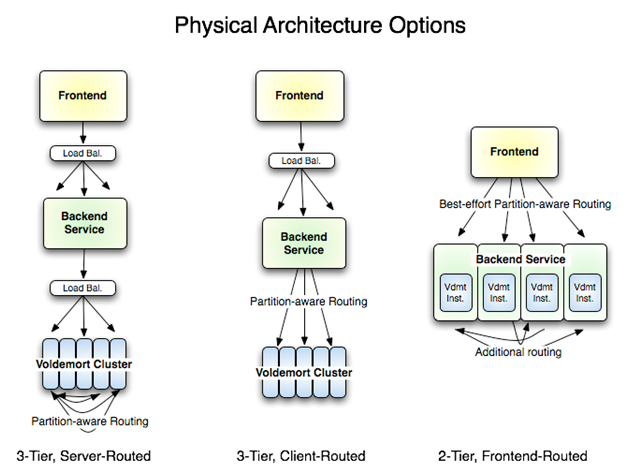
\includegraphics[scale=1]{imgs/voldemort}

Son tres configuraciones diferentes y cada una posee un nivel de decision más. Claramente el de menos niveles es el más rápido y eficiente pero no siempre es posible resolver todas las consultas de forma tal que la lectura se direccione al nodo donde efectivamente se encuentra la información que es requerida o que posea la última actualización disponible, por eso es que existen otras dos configuración que permiten resolver a donde acceder antes de realizar la consulta. Como bien se sabe lo que más cuesta en términos de performance son los accesos a disco y luego la cantidad de procesamiento para la decision de esto, es por eso que encontrar el equilibrio entre ambas lo es importante.\\

\end{subsubsection}

\begin{subsubsection}{Partición y replicación}

La política de partición y replicación de información contenida para las bases de datos es esencial, ya que si la información se concentra en un solo punto este se convierte en un cuello de botellas para las lecturas. Por otro lado, si solo se particiona la información, la caída de cualquier nodo resulta en la instantánea perdida de la información contenida en el. Por esto es tan importante utilizar un criterio adecuado para atacar ambos problemas a la vez.\\

Todos los nodos de la base son independientes entre sí, no posee un coordinador evitando tener un punto de falla.\\

En la base de datos Voldemort se utiliza la técnica de Consistent hashing, una funcion de hash para determinar por Key en que servers se replicará la información de esta. Se toma como input para la función directamente la Key para que sea más facil el buscar donde está contenida la información y de esta forma evitar el tener que guardar una tabla maestra con la informacion de la distribucion en los servers. \\

Un posible ejemplo sería, tenemos la Key A, un total de S servidores y la información se replica en R nodos distintos cuando apliquemos el hash a la Key (hash(A) = H) podemos tomar que desde el servido H hasta el servidor H + R se encuentra replicada la información de la Key A.\\

\end{subsubsection}

\begin{subsubsection}{Modelos y serialización de los datos}

Para Voldemort los datos almacenados, tanto la key como el Value, no son más que un array de bytes. Para darle un formato más alto nivel hay varias opciones de configuración, la aplicación soporta varias pero también da la posibilidad al usuario de generar la propia. Entra las mas usadas estan:\\

\begin{itemize}

\item \textbf{json} - formato alternativo a XML, de fácil uso en javascript.
\item \textbf{string} - solo líneas de string, muy usados para XML blobs.
\item \textbf{java-serialization}
\item \textbf{protobuf} - es un método desarrollado por Google.

\end{itemize}

\end{subsubsection}

\begin{subsubsection}{consistencia y versionado}

Para respaldar la consistencia de los datos, la técnica que Voldemort utiliza es la denominada Read-repair, la cual consiste en no restringir las escrituras sino que el control viene al generarse las lecturas. Se realiza la lectura contra todas las réplicas con esa Key retornando la versión más reciente y replicándose en el resto de las copias. Esto da como resultado que todas las Keys convergen a la versión más actualizada.\\

Si bien este método es aprueba de fallas requiere de un poco más de coordinación y lógica por parte del software.\\

Para el sistema de versionado lo que voldemort utiliza es el algoritmo de vector clocks, un mecanismo muy similar a los relojes de lamport. \\

Este algoritmo consta de llevar ir un reloj o clock y cada vez que se genere un evento incrementar en uno el clock. Cada vez que se necesita versionar algún cambio se asigna el timestamp del clock como versión. Cada vez que llega un cambio con un timestamp mayor al actual, este se pisa con el más grande. \\

Esto da un orden parcial entre las modificaciones y así facilita el resolver los conflictos que puedan llegar a ocurrir.\\

Para dar un orden total solo resta ver cuando se realizan modificaciones simultáneas sobre los datos. Para este caso Voldemort usa bloqueo optimista, es decir, asume que estos casos se dan muy rara vez pero si la comprobación revela modificaciones en conflicto, la transacción que iba a hacer commit hace un rollback y se puede reiniciar.\\

\end{subsubsection}

\end{subsection}

\end{section}
